\documentclass[11pt]{article}
\usepackage[margin=1in]{geometry}
\usepackage[T1]{fontenc}
\usepackage{amsmath,amssymb}
\usepackage{booktabs}
\usepackage{array}
\usepackage{longtable}
\usepackage{graphicx}
\usepackage{placeins}
\usepackage[colorlinks=true,linkcolor=blue,citecolor=blue,urlcolor=blue]{hyperref}

%================================================================
%  The best frequency for inverse bremsstrahlung in excimer laser gases:
%  a krypton fill, the measured 5s to 5p rate, and the pulse.
%  C. K. Watson, 12 October 2026.  Build: latexmk -pdf quant_ib_v4.tex
%  The tables (tab_v4_*.tex), the bibliography (bib_v4.tex), fig_v4_fbest.pdf
%  and Appendix A (qib4_checks.tex) were generated by the scripts that
%  computed the numbers.
%================================================================

\setlength{\emergencystretch}{3em}
\setlength{\LTcapwidth}{\textwidth}
\setlength{\belowcaptionskip}{4pt}
\newcolumntype{L}[1]{>{\raggedright\arraybackslash}p{#1}}
\makeatletter
\newcommand{\tabinput}[1]{\@@input #1 }
\makeatother

\title{The best frequency for inverse bremsstrahlung in excimer laser gases:\\ a krypton fill, the measured 5s to 5p rate, and the pulse}
\author{Cooper K.\ Watson}
\date{October 12, 2026}

\begin{document}
\maketitle

%================================================================
\section{The question and the answer}
\label{sec:answer}
%================================================================

A wave of frequency $f$ heats the electrons of an excimer laser gas by inverse bremsstrahlung. To deposit a power
density $P$ evenly through a layer of depth $L$, it has to be absorbed over that depth and not reflected at the
surface. The best frequency $f_{\rm best}$ is the frequency that does both, defined in Section~\ref{sec:model}. It
depends on the electrons through their temperature and density and on the atoms and ions they collide with, and
the field that heats the electrons also excites the gas. The excited atoms are ionized by a second electron at
under a third of the energy the ground state needs, they ionize each other and the krypton, and they trade energy
with the electrons both ways. This note follows them inside both balances of the electrons, the balance of their
number and the balance of their energy, at every point of a table of three fills, two buffered and one of krypton
with 0.5~\% F$_2$, five pressures and five electron densities, 75 points in all, and it does four things the
earlier form of the calculation could not.

First, the excitation of krypton's 5s levels to 5p, the rate that carries most of the cooling of the electrons,
is taken from the measured cross sections of Jung et al.\ \cite{Jung2005,Jung2006} rather than from a discharge
model's fit, and the 5p manifold radiates to 5s at the measured lifetimes \cite{Dzierzega2000}. Second, the
krypton fill is added, with no buffer gas. Its best frequency lies 1.04 to 1.20 times the argon fill's at the
same pressure and density, 1.05 to 8.8~THz at 0.1~atm and 3.8 to 26.9~THz at 2~atm, with its electrons at 0.94
to 2.44~eV, and the beam holds the density at 11 of its 25 points. With the measured cross section the neon fill
lies at 0.933 to 0.997 and the argon fill at 0.646 to 0.995 of the calculation without excited atoms. The fit in
place of the measurement raises the best frequency by up to 5~\%, the 5p rung's electron collisions left out raise
it by up to 1.46 times, and the return of 5p to 5s by collisions, raised from the estimate used here to the one
measured total loss rate of a 5p level \cite{Gazeli2021}, lowers it by up to 13~\% at the dense krypton points and
the electron temperature there by 19~\%: that return rate is now the largest uncertainty of the answer. Third, the
calculation is marched in time through a pulse of 1~$\mu$s at three points, with the F$_2$ burning and the density
following its own balance. The steady table is the state of the first 100~ns at $10^{15}$~cm$^{-3}$ and of the
first 10~ns at $10^{16}$~cm$^{-3}$: the attachment that holds the density also burns the F$_2$, which is gone in
0.36 to 0.38~$\mu$s at $10^{15}$~cm$^{-3}$ and in 35~ns at $10^{16}$~cm$^{-3}$, after which the density runs up
3.7 to 6.8 times to where the beam's pairs balance recombination, the electrons cool to 0.53 to 0.54~eV and the
best frequency moves, by $-18$ and $-6$~\% at $10^{15}$~cm$^{-3}$ and by 2.8 times at $10^{16}$~cm$^{-3}$. Fourth, the
kinetic solver is checked against a second solver of the same equation, written independently for a time-domain
model of the KrF laser: at seven states from $10^{12}$ to $10^{16}$~cm$^{-3}$ the two agree within 0.2~\% in the
electrons' mean energy and in the wave's absorbed power, and the two full models, started from the same cold seed
under the same wave, decay the plasma at rates 1~\% apart with electrons 0.3~\% apart in temperature.

%================================================================
\section{The gas, the electrons and the best frequency}
\label{sec:model}
%================================================================

\paragraph{The table.}
The three fills are Ne/Kr/F$_2$ in the mole fractions 0.948/0.05/0.002, Ar/Kr/F$_2$ in 0.597/0.4/0.003 and
Kr/F$_2$ in 0.995/0.005, at 300~K and pressures of 0.1, 0.2, 0.5, 1 and 2~atm. The electron density $n_e$ is
$10^{14}$, $3\times10^{14}$, $10^{15}$, $3\times10^{15}$ or $10^{16}$~cm$^{-3}$, and the field deposits
$P=300$~kW/cm$^3$ in a layer of depth $L=10$~cm. At each of these 75 points the frequency runs over 13 values, five
per decade from 0.1 to 25.1~THz.

\paragraph{The electrons.}
The electrons' energy distribution $F(\epsilon)$ solves the two-term Boltzmann equation in the oscillating field
\cite{HP2005}, with the cross sections of Biagi's database for neon, argon, krypton and F$_2$ \cite{LXCat},
electron--electron collisions, and collisions with the cations through the Coulomb cross section
$\pi\,(e^2/4\pi\epsilon_0\epsilon)^2\Lambda(\epsilon,\omega)$. The logarithm $\Lambda$ is the quantum one of
Turnbull et al.\ for the photon energy $\hbar\omega$ \cite{T23,T24}, cut off at the ion-sphere radius of the
cations. The field's amplitude is set so that the electrons absorb $P$. The electrons' complex mobility
$\mu(\omega)$ gives the conductivity $\sigma=n_ee\mu$ and the dielectric function
$\varepsilon=1+i\sigma/\epsilon_0\omega$, and from them the absorption coefficient and the reflection at normal
incidence,
\begin{equation}
\alpha=\frac{2\omega}{c}\,{\rm Im}\sqrt{\varepsilon},\qquad
R=\left|\frac{1-\sqrt{\varepsilon}}{1+\sqrt{\varepsilon}}\right|^2 .
\label{eq:optics}
\end{equation}
$\alpha$ falls with $f$ once $\omega$ exceeds the collision and plasma frequencies. $f_A$ is the frequency at
which $\alpha L=1$, so that the wave is absorbed over the layer, and $f_R$ the lowest at which $R\le0.05$. The
best frequency is
\begin{equation}
f_{\rm best}=\max\left(f_A,\,f_R\right),
\label{eq:fbest}
\end{equation}
both found by interpolating $\ln\alpha$ and $\ln R$ in $\ln f$ between the frequencies of the scan.

\paragraph{The ions and how the density is held.}
Electrons are lost to attachment on F$_2$ and to dissociative recombination on molecular cations. The two buffered
fills have five cations each, the atomic and the molecular ion of the buffer gas, the heteronuclear ion of the
buffer with krypton, Kr$^+$ and Kr$_2^+$, and the krypton fill has Kr$^+$ and Kr$_2^+$. They are made by the
field's ionization of each gas and by an electron beam, they convert into one another, and they recombine with the
electrons and with F$^-$, through the reactions of Table~\ref{tab:ionrows} in Appendix~\ref{app:rows}. The
recombination with F$^-$ turns over with pressure, as the three-body capture calculations that Kannari et al.\
review do \cite{Kannari1985}, and the other charges screen each pair, which multiplies it here by
$S_c=1/(1+R_c/\lambda_D)$ with $R_c=2e^2/(3\cdot4\pi\epsilon_0kT_g)$ and $\lambda_D$ the Debye length of all the
charges at the gas temperature $T_g$. Where the ionization falls short of the losses, the beam makes up the
difference and holds $n_e$. Its electrons enter with the energy spectrum of the slow secondaries of a fast beam,
whose mean is 4.506~eV, and they are marked $b$ where they bring more than a third of the absorbed power. Where
the ionization exceeds the losses, the field multiplies the electrons at the net rate $g$, and the point is marked
$a$ where $g$ exceeds one $e$-fold in the pulse of 1~$\mu$s. A point marked $a$ is not steady over the pulse, and
its best frequency is that of the density it passes through.

%================================================================
\section{The excited atoms}
\label{sec:ladder}
%================================================================

\paragraph{The levels.}
The field excites krypton into its four 5s levels and into 5p and the levels above. They are followed as two
species, Kr$^*$ for the 5s levels and Kr$^{**}$ for 5p and above, each standing at the energy of its lowest level,
9.915 and 11.30~eV, so that no excitation booked into a species creates energy. The buffer gas is followed the same
way, Ar$^*$ at argon's lowest 4s level, 11.548~eV, and Ne$^*$ at neon's lowest 3s level, 16.619~eV, and four
excited dimers form from these atoms, mostly in three-body collisions, Kr$_2^*$, Ar$_2^*$, ArKr$^*$ and Ne$_2^*$.
The krypton fill carries Kr$^*$, Kr$^{**}$ and Kr$_2^*$. Every energy is a formation energy above the ground-state
atoms, Table~\ref{tab:levels}. Those of the atoms lie within 0.005~eV of the levels and ionization limits of the
NIST database \cite{NISTASD}, those of Kr$_2^+$ and Ar$_2^+$ follow from the measured binding of the two ions
\cite{Ng1977}, and the others are taken as the table gives them.

\begin{table}[!tbp]
\centering
\caption{The levels whose energy reaches the electrons, as formation energies above the ground-state atoms, in eV.}
\label{tab:levels}
\small
\begin{tabular}{@{}l r L{8.2cm}@{}}
\toprule
species & energy & origin \\
\midrule
\tabinput{tab_v4_levels.tex}
\bottomrule
\end{tabular}
\end{table}

The field makes Kr$^*$ and Kr$^{**}$ through the excitation cross sections of the Boltzmann equation, the 5s group
into Kr$^*$ and every higher group into Kr$^{**}$, and the buffer's excitations into its own species. The beam
shares its energy between the gases by their stopping powers for fast electrons, from Bethe's formula at 600~keV
with mean excitation energies of 137, 188, 352 and 115~eV for Ne, Ar, Kr and F$_2$, and makes one ion pair per
36.6~eV in neon \cite{Lee1989}, 26.2~eV in argon and 32~eV in F$_2$ \cite{Kannari1985}, and 24.2~eV in krypton,
where Kannari et al.\ print 24.3. With each pair it makes 0.305 excited atoms in neon and 0.284 in argon, the
energies per pair of Lee et al.\ over their energies per excited atom, 120 and 93~eV \cite{Lee1989}, and 0.28 in
krypton \cite{Kannari1985}. The recombination of the molecular cations leaves an excited atom behind. The excited
atoms are lost to F$_2$, which turns Kr$^*$ into KrF$^*$ at $8.47\times10^{-10}$~cm$^3$\,s$^{-1}$, the mean of
three measurements, with a yield of 0.90 \cite{Velazco1976,Ueda1984}, to the three-body formation of dimers, to
radiation, to Penning ionization, and to the electrons. Tables~\ref{tab:hrows} and \ref{tab:ionrows} of
Appendix~\ref{app:rows} list every reaction between heavy particles with its rate and its source, and
Table~\ref{tab:erows} the electron collisions. Each species stands at the steady state of its balance, solved for
all of them at once at the electrons' distribution. Where the field multiplies the electrons at the rate $g$, every
density grows with them, the ions as the excited atoms, and each species is diluted at $gn$ on top of its losses.

\begin{table}[!htbp]
\centering
\caption{The electron collisions of the excited atoms as the Boltzmann equation carries them. The rate is the
source's in cm$^3$\,s$^{-1}$ with $T_e$ in eV, $E_0$ the onset of the cross section of Eq.~(\ref*{eq:sigma}) in eV,
and $\Delta$ the energy the electron loses, negative where it gains. The standing says whether the rate is measured,
printed by its source from elsewhere, calculated, the value of a related process, estimated, or detailed balance.}
\label{tab:erows}
\footnotesize
\setlength{\tabcolsep}{3pt}
\begin{tabular}{@{}L{3.6cm} L{3.7cm} r r L{1.6cm} L{3.4cm}@{}}
\toprule
reaction & rate & $E_0$ & $\Delta$ & standing & source \\
\midrule
\tabinput{tab_v4_erows.tex}
\bottomrule
\end{tabular}
\end{table}

\paragraph{The 5s to 5p excitation is measured.}
Jung et al.\ measured the cross sections for electron-impact excitation out of krypton's two metastable 5s
levels, $1s_5$ and $1s_3$ in Paschen's notation, into each of the ten 5p levels, from 2 to 300~eV, with
uncertainties of 35~\% for $1s_5$ and 40~\% for $1s_3$ \cite{Jung2005,Jung2006}. The cross section used here for
Kr$^*\to$ Kr$^{**}$ is their sum over the ten 5p levels, lumped over the 5s manifold by statistical weight,
$1s_5:1s_4:1s_3:1s_2=5:3:1:3$, with each unmeasured resonance level taken as its core partner, $1s_4$ as $1s_5$
and $1s_2$ as $1s_3$, since the core-preserving cross sections scale with the optical oscillator strengths. Each
level's cross section is zero below its threshold, rises linearly to the first tabulated point, follows the table
log-log between the points, and falls as $1/\epsilon$ past the last. Its onset on the ladder is the gap
between the lumped levels, 1.385~eV. On Maxwellians this cross section gives 1.36 times the rate of the discharge
model's fit that Kannari et al.\ print \cite{Kannari1985,JacobMangano1976} at the coldest electrons of the table,
0.87~eV, and 0.92 times at the hottest, 4.69~eV, differences at or inside the measurement's own uncertainty. The
fit is kept as the upper end of a band, Section~\ref{sec:limits}.

\paragraph{The 5p manifold returns to 5s three ways.}
Kr$^{**}$ gives its energy back to the electrons in superelastic collisions, the detailed balance of the
excitation, and it returns to 5s by radiation and in collisions with the gas. The ten 5p levels radiate to the 5s
levels in the near infrared, on lines that end on the 5s levels and are not trapped, with the lifetimes that
Dzierzega et al.\ derive from the beam-gas-laser measurements of six of the levels, 23.1 to 38.1~ns
\cite{Dzierzega2000}. The lumped manifold decays at the $2J+1$-weighted mean of their rates, one lifetime of
29.0~ns, and the 1.385~eV leaves as light. The return by collisions is the estimate of
$1.0\times10^{-10}$~cm$^3$\,s$^{-1}$ that Kannari et al.\ mark as such for Kr$^{**}$ + Ar \cite{Kannari1985},
used for every partner. One measurement in krypton exists: Gazeli et al.\ measured the total loss rate of the
$5p'[3/2]_2$ level in krypton at 300~K, $(1.7\pm0.2)\times10^{-10}$~cm$^3$\,s$^{-1}$, without resolving its
product \cite{Gazeli2021}. It bounds the return of the lumped manifold from above and is run as the upper end of
a band. The level-resolved rates of Whitehead et al.\ \cite{Whitehead1995} would settle it and are not used
here. At the krypton fill at 1~atm and $10^{15}$~cm$^{-3}$, at 10~THz, the manifold returns 84~\% by collisions,
15~\% superelastically and 1.2~\% by radiation.

\paragraph{Stepwise ionization has no measurement.}
No measurement of the ionization of krypton's 5s levels by electrons was found, as a cross section or as a rate.
Kannari et al.\ print $7.00\times10^{-8}\,T_e^{0.68}e^{-4.04/T_e}$~cm$^3$\,s$^{-1}$ for it from Vriens's
binary-encounter calculation \cite{Kannari1985,Vriens1965}, and Johnson and Hunter print $4.8\times10^{-8}$ from
the same calculation \cite{JH1980}. This note takes Kannari's fit. The stepwise ionization of Ar$^*$ has only a
transplanted law, that of Chen et al.\ for the higher of their two excited argon species
\cite{Chen2025} at argon's 4s binding energy. In the calculation with Kannari's 5s to 5p fit, a stepwise rate
2.1 to 2.3 times Kannari's, or none at all, moved the best frequency by less than 1.5~\%, so the answer does not
rest on this rate and no band is run on it here.

%================================================================
\section{The excited atoms inside the electrons' balances}
\label{sec:loop}
%================================================================

\paragraph{Every electron collision of an excited atom is a process of the Boltzmann equation.}
Each excited species enters the Boltzmann equation as a gas of its own, at the mole fraction its balance gives,
with every collision of an electron with it that Table~\ref{tab:erows} lists. A rate fitted as $k=A\,T^B e^{-E/T}$
becomes the cross section
\begin{equation}
\sigma(\epsilon)=C\,\frac{(\epsilon-E_0)^{B+1/2}}{\epsilon}\quad(\epsilon>E_0),\qquad
C=\frac{A\sqrt{\pi}}{2\gamma\,\Gamma(B+3/2)},
\label{eq:sigma}
\end{equation}
with $\gamma=(2e/m_e)^{1/2}$, whose rate over a Maxwellian of temperature $T$ is exactly $A\,T^Be^{-E_0/T}$. The
electron loses in it the energy $\Delta$ of the reaction on the ladder of formation energies of
Table~\ref{tab:levels}. An electron below $\Delta$ cannot pay it, so the onset $E_0$ is the larger of the fit's $E$
and $\Delta$. Where the fit's $E$ lies above $\Delta$ the printed rate is kept and the electron loses $\Delta$.
Where it lies below, the onset moves up to $\Delta$, which lowers the rate on a Maxwellian by $e^{-(\Delta-E)/T}$.
A constant rate $k$ is the cross section $k/\gamma\sqrt{\epsilon}$, and a measured cross section enters as it is,
above the ladder's gap.

\paragraph{De-excitation by detailed balance.}
In a superelastic collision the electron gains the energy $\Delta$ of the level it empties. Its cross section
follows from that of the excitation it reverses by detailed balance \cite{KR1921},
\begin{equation}
\sigma_{\downarrow}(\epsilon)=\frac{g_l}{g_u}\,\frac{\epsilon+\Delta}{\epsilon}\,\sigma_{\uparrow}(\epsilon+\Delta),
\label{eq:db}
\end{equation}
with $g_l$ and $g_u$ the statistical weights of the lower and the upper level. Over a Maxwellian its rate is
$(g_l/g_u)\,e^{\Delta/T}$ times that of the excitation, and when the electrons are in equilibrium with the excited
atoms the two flows cancel. The Boltzmann operator places the electron $\Delta$ above the energy it had, so that
the equation is no longer solved from the top of the energy grid down and is solved as one linear system.

\paragraph{The electrons that the excited atoms set free.}
Penning ionization, between two excited atoms or dimers or between one of them and ground-state krypton, releases
an electron with the energy that the reaction leaves on the ladder, from 2.1 to 12.0~eV. These electrons enter the
Boltzmann equation as a source at their release energy, each in a band 0.2~eV wide.

\paragraph{The two closures.}
The Boltzmann equation is solved in steady state with a source of electrons. Where the beam holds the density, the
source is the beam's slow secondaries and the Penning electrons, mixed in proportion to their rates, and the rate
of injection per electron is what the losses leave over,
\begin{equation}
s=N\left(k_{\rm att}+k_{\rm rec}-k_{\rm ion}\right)=\frac{S_{\rm beam}+S_{\rm pen}}{n_e},
\label{eq:held}
\end{equation}
with $N$ the gas density and $k_{\rm ion}$ the ionization of every gas of the equation, the excited ones among
them. Where the field multiplies the electrons at the rate $g$, the Penning electrons are the source and $g$ enters
as a loss from every energy in proportion to the electrons there, the dilution that growth brings, set so that
\begin{equation}
N\left(k_{\rm att}+k_{\rm rec}-k_{\rm ion}\right)+g=\frac{S_{\rm pen}}{n_e}.
\label{eq:grow}
\end{equation}
Without a source the second closure is the growth model of the two-term equation \cite{HP2005}. It leaves out the
share of the growth term in the anisotropic part of the distribution, which is of the order of $g/\nu_m$, the
growth rate over the momentum-transfer frequency, below $3\times10^{-3}$ at every growing point. The cations
follow the same particle balance, with the excited atoms' stepwise electrons added to the ionization of their
ground gas and the dimers' and the Penning electrons to their own cations.

\paragraph{The loop.}
Each round solves the Boltzmann equation with the excited atoms at their current mole fractions, then their
balance with the rates over the new distribution, then the ions, and sets the closure and the source of the next
round. The mole fractions are relaxed in their logarithm, and the loop ends when they, the ions and the beam's or
the growth rate change by less than $2\times10^{-3}$ between two rounds and the closure no longer changes. A
growth rate's change is measured against the larger of itself and $10^6$~s$^{-1}$, one $e$-fold in the pulse,
below which a growth rate multiplies nothing and its relative change says nothing. At the boundary between the
closures the two can alternate from round to round, with the beam's rate alternating between zero and a finite
value and the excited atoms differing by up to 1~\% between the two states, which is one and the same plasma within
that: a point whose excited atoms and ions have settled within ten tolerances and whose closure has alternated
for three rounds is accepted and flagged as a boundary point. It took 3 to 72 rounds per point, the most at the
one boundary cell of Section~\ref{sec:limits}. Each frequency starts from the state of the one below it. The
electrons and the excited atoms book the same energy for every collision, which Appendix~\ref{app:checks} tests
row by row as an identity.

%================================================================
\section{Results}
\label{sec:results}
%================================================================

\paragraph{The table.}
Table~\ref{tab:fbest} and Figure~\ref{fig:fbest} give the best frequency at the 75 points with the excited atoms
inside the electrons' balances and the measured 5s to 5p cross section, and Table~\ref{tab:compare} of
Appendix~\ref{app:compare} every point with its electron temperature, its marks, the mole fraction of Kr$^*$, the
net energy the excited atoms take from the electrons, and the bands of Section~\ref{sec:limits}. One cell of the
krypton fill, 0.5~atm and $10^{14}$~cm$^{-3}$, is a marginal plasma whose two closures alternate at most of its
frequencies, with the excited atoms moving by more than the boundary rule allows: 9 of its 13 frequencies closed,
4 of them at the flipping boundary, and the cell is reported incomplete, blank in the table and the figure and left
out of the bands.

\begin{table}[!tbp]
\caption{The best frequency $f_{\rm best}$ in THz at $L=10$~cm and 300~kW/cm$^3$ with the excited atoms inside the
electrons' balances. Marked $a$ where the field multiplies the electrons more than $e$-fold in the pulse of
1~$\mu$s, and $b$ where the beam's electrons bring more than a third of the absorbed power.}
\label{tab:fbest}
\centering
\begin{tabular}{llrrrrr}
\toprule
fill & $p$ [atm] & $n_e=10^{14}$ & $3\times10^{14}$ & $10^{15}$ & $3\times10^{15}$ & $10^{16}$~cm$^{-3}$\\
\midrule
\tabinput{tab_v4_fbest.tex}
\bottomrule
\end{tabular}
\end{table}

\begin{figure}[!tbp]
\centering
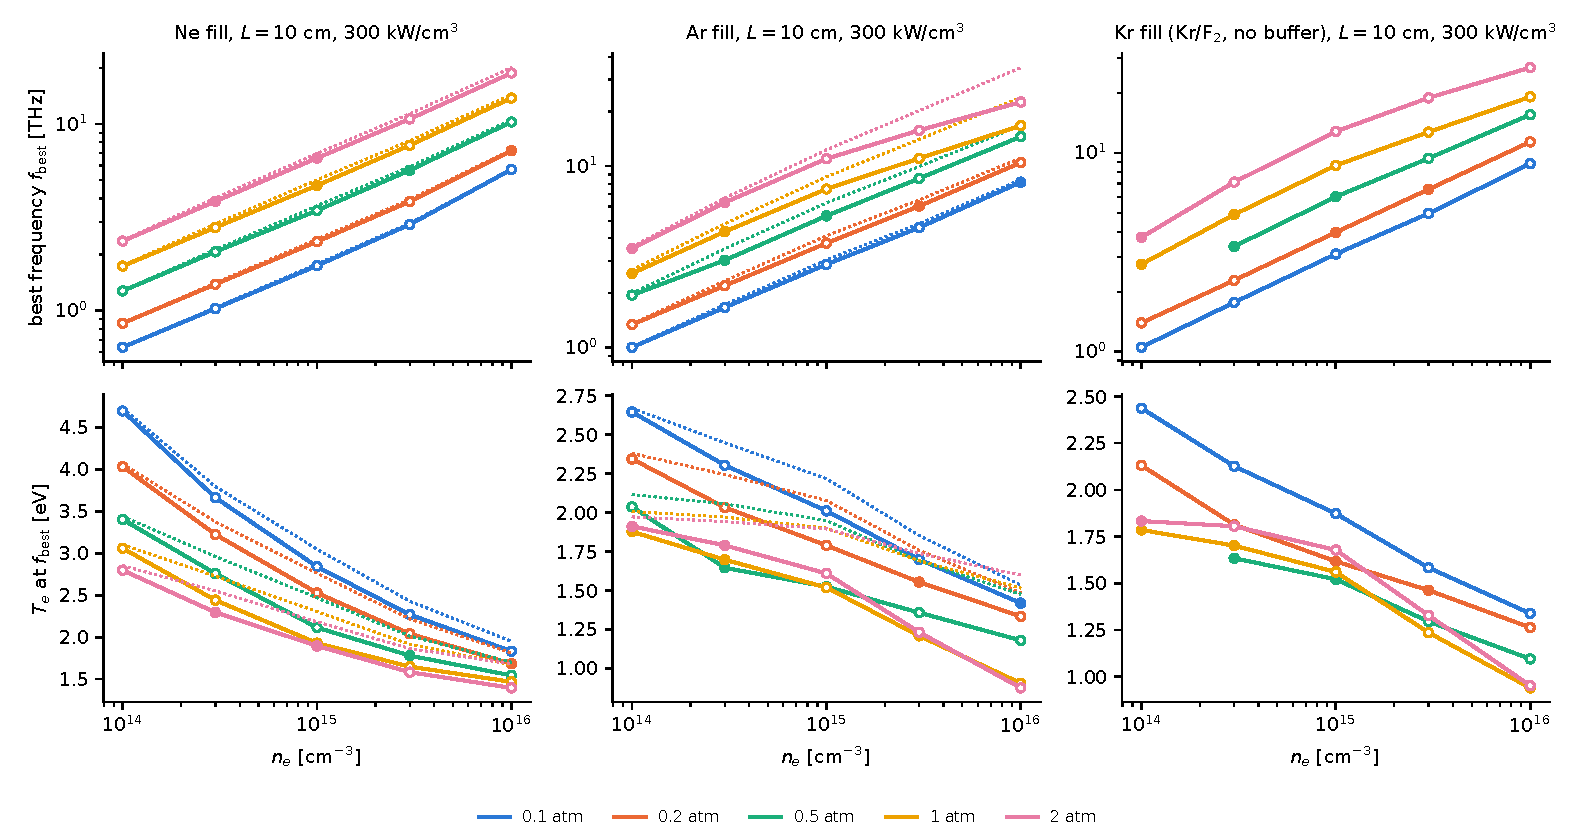
\includegraphics[width=\textwidth]{fig_v4_fbest.pdf}
\caption{The best frequency at $L=10$~cm and 300~kW/cm$^3$ against $n_e$, top, and the electron temperature
$2\langle\epsilon\rangle/3$ there, bottom, with the excited atoms as solid lines and, for the two buffered fills,
without them dotted. An open marker is a point marked $a$ or $b$ in Table~\ref{tab:fbest}. The krypton fill's cell
at 0.5~atm and $10^{14}$~cm$^{-3}$ is left blank.}
\label{fig:fbest}
\end{figure}

\paragraph{The krypton fill against the argon fill.}
At the same pressure and density the krypton fill's best frequency lies 1.04 to 1.20 times the argon fill's, the
least at 0.2~atm and $3\times10^{14}$~cm$^{-3}$ and the most at 2~atm and $3\times10^{15}$~cm$^{-3}$. The reason
is the collision frequency. Above the collision frequency $\alpha$ falls as $\nu_m/\omega^2$, so the frequency at
which $\alpha L=1$ scales as the square root of the effective momentum-transfer frequency
$\nu_m=\omega\mu_r/\mu_i$, the ratio of the real to the imaginary part of the mobility times $\omega$. At the best
frequencies $\nu_m$ of the krypton fill is 1.08 to 1.52 times the argon fill's, and its square root gives the ratio
of the best frequencies within 3.5~\%. Krypton's momentum-transfer cross section rises from 0.54 of argon's at
1~eV to 1.55 times at 3~eV \cite{LXCat}, and the argon fill is 40~\% krypton. The electrons of the krypton fill sit
at 0.94 to 2.44~eV, those of the argon fill at 0.87 to 2.65~eV and those of the neon fill at 1.40 to 4.69~eV.

\paragraph{How the density is held.}
The field multiplies the electrons at 15 points of the neon fill, 8 of the argon fill and 6 of the krypton fill,
marked $a$, and the beam brings more than a third of the absorbed power at 5, 9 and 11, marked $b$. The excited
atoms take from the electrons, net of what they give back in superelastic collisions, 0.007 to 2.9 times the
absorbed power in the neon fill, 0.012 to 15.0 times in the argon fill and 0.017 to 23.5 times in the krypton fill,
the most at 2~atm and $10^{16}$~cm$^{-3}$ in each. Where they take more than the field gives, the beam holds the
density and its slow electrons bring the difference. With the measured cross section the best frequency of the
neon fill lies at 0.933 to 0.997 of its value without the excited atoms and that of the argon fill at 0.646 to
0.995, falling at every point, by the most at 2~atm and $10^{16}$~cm$^{-3}$ in the argon fill, from 34.9 to
22.5~THz. The electrons there are at 0.55 to 0.99 of their temperature without the excited atoms in the argon fill
and 0.83 to 0.99 in the neon fill. The krypton fill has no counterpart without excited atoms.

%================================================================
\section{What limits the answer}
\label{sec:limits}
%================================================================

\paragraph{Three bands.}
Three more scans of the 75 points bound what the rates of the 5p rung can do, Table~\ref{tab:compare}. With
Kannari's fit in place of the measured 5s to 5p cross section the best frequency rises to 1.000 to 1.049 times the
reference, up to 1.010 in the neon fill, 1.047 in the argon fill and 1.049 in the krypton fill, the most at 2~atm
and $10^{16}$~cm$^{-3}$, where the krypton fill moves from 26.9 to 28.2~THz, with the electrons hotter by at most
6.7~\%. With every electron collision of the 5p rung left out, so that collisions and radiation alone return
Kr$^{**}$ to 5s, it rises to 1.00 to 1.46 times the reference, up to 1.054 in the neon fill, 1.460 in the argon
fill and 1.436 in the krypton fill, the most at 2~atm and $10^{16}$~cm$^{-3}$ in the argon fill, where it returns
to 32.9~THz: the 5s to 5p cycle carries the fall. With the return of 5p to 5s by collisions raised from Kannari's
estimate to the measured total loss rate of Gazeli et al., $1.7\times10^{-10}$~cm$^3$\,s$^{-1}$, it falls to 0.868
to 1.000 times the reference, to 0.999 in the neon fill, 0.951 in the argon fill and 0.868 in the krypton fill, the
most at 0.5~atm and $10^{16}$~cm$^{-3}$ in the krypton fill, where it moves from 15.6 to 13.5~THz with the
electrons at 0.81 of their reference temperature. A faster return empties the 5p manifold before the electrons can
ionize it or take their energy back, so more of the energy of the cycle ends in the gas and the electrons are
colder. The return rate by collisions is thus the largest uncertainty of the answer at the dense krypton points,
13~\% in the best frequency and 19~\% in the electron temperature, and a level-resolved measurement in krypton
\cite{Whitehead1995} would replace it.

\paragraph{What the model leaves out.}
Kr$^{**}$ lumps 5p and the levels above at the lowest 5p level, and argon and neon have no second rung. The four
argon levels give back up to 0.28~eV more in superelastic collisions than the lumped Ar$^*$ holds. The growing
closure leaves out a share of order $g/\nu_m<3\times10^{-3}$ in the anisotropic part of the distribution, one
point of the argon fill lies on the boundary between the closures and one cell of the krypton fill is incomplete.
The recombination of Kr$_2^+$ puts the sum of the two branches that Kannari et al.\ print at 300~K on a
$T_e^{-1/2}$ law \cite{Kannari1985}. The excited atoms settle within 220~ns, but the gas is held at its fill
composition, while attachment alone would take the F$_2$ down $e$-fold in 24 to 56~ns at $10^{16}$~cm$^{-3}$ and
in 0.44 to 0.97~$\mu$s at $10^{15}$~cm$^{-3}$. What that means for the table is the subject of the next section.

%================================================================
\section{The pulse}
\label{sec:pulse}
%================================================================

\paragraph{The march.}
The steady state of the table is marched in time at three of its points. The kinetic solution of the electrons is
renewed every few nanoseconds: whenever the slowest of the electron density, the F$_2$ and the excited atoms would
move by 2~\%, at least every 10~ns, 5~ns in the third pulse, until a twentieth of the time elapsed exceeds that,
and every twentieth of the time elapsed after, and between renewals the excited species, the cations, F$^-$ and F$_2$ are
integrated with the renewed rate coefficients held, the electron density following from quasineutrality. The
F$_2$ burns by attachment, by the harpoon reactions of the excited atoms and by its own ionization. At each renewal
the field is solved again so that the wave deposits $P$, the solve carries the electrons' sources, the beam's
secondaries and the Penning electrons at their release energies, and the instantaneous net rate $g$ of the density
enters as the uniform loss of Eq.~(\ref{eq:grow}), given rather than solved, so that the distribution's shape is
that of a plasma changing at that rate. The beam is a constant current, at the pair rate that held the density at
the point's steady state at $t=0$. Held still are the gas temperature, 300~K, the atomic fluorine beyond the
consumption of F$_2$, the excimers, which are sinks, and the buffer and krypton densities. At chosen times the
13-frequency scan is solved at the frozen state and the best frequency of that state found by the definitions of
Section~\ref{sec:model}.

\begin{table}[!tbp]
\caption{Three pulses at 300~kW/cm$^3$, the beam holding the density at $t=0$: the electron density in cm$^{-3}$,
the electron temperature in eV, the mole fraction of Kr$^*$ in units of $10^{-4}$, the F$_2$ over its fill value,
the net rate $g$ of the density in $10^6$~s$^{-1}$, the rms field in kV/cm and the absorption coefficient in m$^{-1}$
at the wave's frequency.}
\label{tab:pulse}
\centering
\small
\begin{tabular}{@{}rrrrrrrr@{}}
\toprule
$t$ [ns] & $n_e$ & $T_e$ & $x_{{\rm Kr}^*}$ & F$_2$ & $g$ & $E$ & $\alpha$ \\
\midrule
\tabinput{tab_v4_pulse.tex}
\bottomrule
\end{tabular}
\end{table}

\begin{table}[!tbp]
\caption{The best frequency in THz of the frozen state at the checkpoints of the three pulses, with $f_R$ in
parentheses.}
\label{tab:fbest_t}
\centering
\small
\begin{tabular}{@{}lrrrrr@{}}
\toprule
pulse & 0~ns & 30~ns & 100~ns & 300~ns & 1000~ns \\
\midrule
\tabinput{tab_v4_fbest_t.tex}
\bottomrule
\end{tabular}
\end{table}

\paragraph{What the pulses say.}
Table~\ref{tab:pulse} follows the krypton fill and the argon fill at 1~atm and $10^{15}$~cm$^{-3}$ at the
table's best frequencies, 10 and 7.7~THz, and the krypton fill at 1~atm and $10^{16}$~cm$^{-3}$ at its own,
19.2~THz, and Table~\ref{tab:fbest_t} the best frequency of the frozen state at the checkpoints. The attachment
that holds the density burns the F$_2$ at $3\times10^{8}$ to $6\times10^{8}$ molecules per electron per second. At
$10^{15}$~cm$^{-3}$ half of it is gone at 134~ns and all but 1~\% by 365~ns in the krypton fill and 383~ns in the
argon fill. The density then runs up, 3.75 times in the krypton fill and 3.95 times in the argon fill, until the
beam's pairs balance recombination, which they do by 0.44 to 0.47~$\mu$s, the same power spread over four times
the electrons cools them from 1.56 and 1.52~eV to 0.535 and 0.542~eV, Kr$^*$ accumulates 10 and 8 times once its
harpoon partner is gone, and the field for the same deposited power rises from 38.9 to 47.6~kV/cm in the krypton
fill. The best frequency of the plasma rises at first, by 2 and 3~\% at 100~ns, then falls, to 0.82 and 0.94 of
its start at 1~$\mu$s. At 100~ns the density is up by 25 and 28~\%, the electrons are at 1.37 and 1.34~eV and the
F$_2$ at 0.61 and 0.60 of its fill, so the state of the table holds, within 3~\% in the best frequency, for the
first 100~ns at this density. At $10^{16}$~cm$^{-3}$ half of the F$_2$ is gone at 11~ns and all but 1~\% at
35~ns, the density runs up 6.8 times by 92~ns, the electrons cool from 0.94 to 0.53~eV, the field for the same
power falls from 33.6 to 12.1~kV/cm as $\alpha$ at 19~THz climbs from 10.0 to 78~m$^{-1}$, so that the wave then
stops within 1.3~cm of the 10-cm layer, and the best frequency of the new plasma is 1.52 times the table's at 30~ns
and 2.75 times, 53~THz, from 100~ns on. At 10~ns the density is up by 32~\% and the F$_2$ at 0.54 of its fill: at
$10^{16}$~cm$^{-3}$ the table's answer holds for the first 10~ns. A shorter pulse, a lower beam current or more
F$_2$ keeps the table's answer longer, and the march gives the time it holds at any point.

%================================================================
\section{The kinetic solver against a second solver}
\label{sec:solvers}
%================================================================

\paragraph{The same equation twice.}
The two-term Boltzmann equation of Section~\ref{sec:model}, with its wave term, its electron--electron term, its
growth closure and the electron--ion absorption of Turnbull et al., was solved a second time by a solver written
independently for a time-domain model of the KrF laser, with its own implementation of the Turnbull construction
from the same two papers \cite{T23,T24} and the same cross sections \cite{LXCat}. Table~\ref{tab:solvers} compares
the two on the krypton fill at seven states, from $10^{12}$ to $10^{16}$~cm$^{-3}$, 0.1 to 1~atm and 95~GHz to
10~THz, with the ions carrying from none to a quarter of the absorption: a given rms field and frequency, no
excited atoms, no sources, the net frequency of ionization and attachment self-consistent in both, the second
solver started from the first's converged distribution. The mean energies agree within 0.2~\%, the wave's absorbed
power within 0.2~\% and the net frequency within 0.6~\% at every state. The share of the absorption the two book
to the ions differs by definition at 95~GHz, 0.19 against 0.17 at 0.1~atm and $10^{16}$~cm$^{-3}$, while the
total power agrees to 0.02~\%: the first books the ions' part by their share of the momentum transfer in the
field term, the second re-evaluates the field term with the atoms' momentum transfer alone, and below
$\omega\sim\nu_m$ that is not the complement. The optics of Eq.~(\ref{eq:optics}) computed on the second solver's
distributions, from the same momentum-transfer sum its wave term uses, give $\alpha$ within 0.2~\% and $R$ within
0.4~\% of the first's at the seven states, over $\alpha$ from 2.3 to $3.4\times10^{4}$~m$^{-1}$ and $R$ from
$3\times10^{-8}$ to 0.91, and the power the mobility implies equals the second solver's own absorbed power to
$10^{-4}$. The absorption that defines the best frequency is therefore the same in both.

\begin{table}[!tbp]
\caption{The two kinetic solvers at one and the same state of the krypton fill: the rms field in kV/cm, the
reduced field in Td, the mean energy in eV, first solver / second solver, the ratio of the wave's absorbed power
per electron, second over first, the share of the absorption each books to the ions, and the ratio of the net
frequency of ionization and attachment, second over first.}
\label{tab:solvers}
\centering
\small
\begin{tabular}{@{}llrlrlrlr@{}}
\toprule
$p$ [atm] & $n_e$ [cm$^{-3}$] & $E$ & $f$ & $E/N$ & $\langle\epsilon\rangle$ & $P_2/P_1$ & ions' share & $\nu_2/\nu_1$ \\
\midrule
\tabinput{tab_v4_solvers.tex}
\bottomrule
\end{tabular}
\end{table}

\paragraph{The two full models from the same cold start.}
The second solver belongs to a time-domain model of the KrF laser that evolves the gas temperature, the excimers,
the photons and the walls as well as the species followed here. The two full models were started from one and the
same state, the krypton fill at 1~atm with a seed of $10^{15}$ electrons/cm$^3$ and as many Kr$^+$, no excited
atoms, no F$^-$, under a wave of 38.9~kV/cm rms at 10~THz, the field the table needs for 300~kW/cm$^3$ at this
point, and no beam, and run for 100~ns, Table~\ref{tab:cold}. Without a beam, attachment outruns the wave's own
ionization at this fill and both models decay the plasma: the second model at $2.17\times10^{8}$~s$^{-1}$ between 10
and 100~ns, the march of Section~\ref{sec:pulse} at $2.15\times10^{8}$~s$^{-1}$ from 40~ns on, 1~\% apart, with the
electrons of the decaying plasma at 1.747 and 1.742~eV, 0.3~\% apart. The two differ only in the first 10~ns, where
the second model heats its seed from the gas temperature and loses three decades of density to the attachment of
the still-cold electrons on the way, while the march starts from the distribution solved hot at $t=0$. The second
model burns 0.9~\% of the F$_2$, the march 1.4~\%, the difference again in the first 10~ns, and the gas warms by
3.4~K in the second model while the march holds it at 300~K.

\begin{table}[!tbp]
\caption{The two full models from the same cold start, the krypton fill at 1~atm under 38.9~kV/cm at 10~THz with
no beam: the electron density in cm$^{-3}$, the electron temperature in eV and the Kr$^*$ density in cm$^{-3}$,
each second model / march, the F$_2$ over its fill value in both, and the second model's gas temperature in K.}
\label{tab:cold}
\centering
\small
\begin{tabular}{@{}rrrrrrrrrr@{}}
\toprule
$t$ [ns] & $n_e$, second & march & $T_e$, second & march & Kr$^*$, second & march & F$_2$, second & march & $T_g$ \\
\midrule
\tabinput{tab_v4_cold.tex}
\bottomrule
\end{tabular}
\end{table}

%================================================================
\section{Where the calculation stands}
\label{sec:stands}
%================================================================

The best frequency of Table~\ref{tab:fbest} rests on the measured 5s to 5p cross section, on the measured
lifetimes of the 5p levels, on an estimate for the return of 5p to 5s by collisions that one measured total loss
rate bounds, and on a calculated stepwise ionization that the answer does not rest on. Its largest uncertainty is
the return rate, 13~\% in the best frequency and 19~\% in the electron temperature at the dense krypton points,
and a level-resolved measurement would remove it. The table is the state of the first 100~ns of a beam-held pulse
at $10^{15}$~cm$^{-3}$ and of the first 10~ns at $10^{16}$~cm$^{-3}$, after which the F$_2$ is gone and the best
frequency of the plasma that remains is the march's, not the table's. The kinetic solver behind both agrees with an
independent one to 0.2~\%. What the calculation still leaves out, the gas temperature, the excimers' own kinetics
and the photons, the atomic fluorine and the walls, belongs to the time-domain model the second solver was written
for, and the next step is to carry the absorption of Eq.~(\ref{eq:optics}) and the excited atoms' electron
collisions of Table~\ref{tab:erows} into it.

\FloatBarrier
\appendix
\section{The checks}
\label{app:checks}

Every number of this note and every step of the calculation behind it is tested by the checks listed in
Table~\ref{tab:checks}, which end with all of them passing. Section K tests the electron collisions of the excited
atoms: each fitted process against its source's printed rate on Maxwellians, the measured cross section against
its tables and its own integral, each de-excitation against detailed balance, every energy against the ladder, the
5p lifetime against the ten level lifetimes, and the identity that the energy the excited atoms take from the
electrons equals the sum, over the collisions the Boltzmann equation carries, of their events times the energy
each takes. Section C checks every point of the four scans: each must close the same way for the electrons and the
ions, the two energy books must agree, the residuals must be small, and one point is solved again in a fresh
process. Section B recomputes a best frequency from the scan. Section L checks the comparison with the second
solver and section P the pulses, their quasineutrality, the monotone burn of the F$_2$ and their checkpoints.
Section N computes every number the text prints from the data, section E ties each printed number and claim to
them, and section S checks the style and that no file or unpublished note is named.

\begingroup
\small
\setlength{\tabcolsep}{4pt}
\begin{longtable}{@{}r L{3.1cm} L{6.6cm} L{3.4cm} l@{}}
\caption{The checks of this note.}\label{tab:checks}\\
\toprule
& check & what & value & \\
\midrule
\endfirsthead
\toprule
& check & what & value & \\
\midrule
\endhead
\tabinput{qib4_checks.tex}
\bottomrule
\end{longtable}
\endgroup

\section{The rows}
\label{app:rows}

The heavy-particle reactions of the excited atoms, Table~\ref{tab:hrows}, at 300~K, and the reactions of the
cations, Table~\ref{tab:ionrows}, in SI units as the ion balance takes them, m$^3$\,s$^{-1}$ for two bodies and
m$^6$\,s$^{-1}$ for three, with $T_e$ in eV. F$(a,s)$ is $aN/(N^2+1.7)\,s$ and L$(A,b,c)$ is $AN/(N^2+bN+c)$, both
in cm$^3$\,s$^{-1}$ with $N$ in amagat. A rate run as a band stands at its default.

\begingroup
\footnotesize
\setlength{\tabcolsep}{3pt}
\begin{longtable}{@{}L{4.6cm} L{3.6cm} L{1.7cm} L{5.6cm}@{}}
\caption{The heavy-particle reactions of the excited atoms.}\label{tab:hrows}\\
\toprule
reaction & rate & standing & source \\
\midrule
\endfirsthead
\toprule
reaction & rate & standing & source \\
\midrule
\endhead
\tabinput{tab_v4_hrows.tex}
\bottomrule
\end{longtable}

\begin{longtable}{@{}L{4.6cm} L{3.6cm} L{1.7cm} L{5.6cm}@{}}
\caption{The reactions of the cations.}\label{tab:ionrows}\\
\toprule
reaction & rate & standing & source \\
\midrule
\endfirsthead
\toprule
reaction & rate & standing & source \\
\midrule
\endhead
\tabinput{tab_v4_ionrows.tex}
\bottomrule
\end{longtable}
\endgroup

\section{Every point}
\label{app:compare}

\begingroup
\footnotesize
\setlength{\tabcolsep}{3pt}
\begin{longtable}{@{}llrrrlrrrrrr@{}}
\caption{The 75 points at $L=10$~cm and 300~kW/cm$^3$ with the excited atoms inside the electrons' balances and the
measured 5s to 5p cross section: the best frequency in THz, the electron temperature at it in eV, the marks of
Table~\ref{tab:fbest}, the mole fraction of Kr$^*$ in units of $10^{-4}$, the net energy the excited atoms take from
the electrons over the absorbed power, then the best frequency of each band over this one, with Kannari's fit in
place of the measured cross section ($k$), with the 5p rung's electron collisions left out ($5p$) and with the
collisional return of 5p at the measured bound ($r$), and the best frequency over the calculation without excited
atoms where that exists ($f/f_0$).}\label{tab:compare}\\
\toprule
fill & $p$ & $n_e$ & $f_{\rm best}$ & $T_e$ & & $x_{{\rm Kr}^*}$ & $p_{\rm net}/P$ & $k$ & $5p$ & $r$ & $f/f_0$ \\
\midrule
\endfirsthead
\toprule
fill & $p$ & $n_e$ & $f_{\rm best}$ & $T_e$ & & $x_{{\rm Kr}^*}$ & $p_{\rm net}/P$ & $k$ & $5p$ & $r$ & $f/f_0$ \\
\midrule
\endhead
\tabinput{tab_v4_compare.tex}
\bottomrule
\end{longtable}
\endgroup

\begin{thebibliography}{99}
\tabinput{bib_v4.tex}
\end{thebibliography}
\end{document}
